%File: formatting-instructions-latex-223.tex
%release 223.
\documentclass[letterpaper]{article} % DO NOT CHANGE THIS
\usepackage{aaai23}  % DO NOT CHANGE THIS
\usepackage{times}  % DO NOT CHANGE THIS
\usepackage{helvet}  % DO NOT CHANGE THIS
\usepackage{courier}  % DO NOT CHANGE THIS
\usepackage[hyphens]{url}  % DO NOT CHANGE THIS
\usepackage{graphicx} % DO NOT CHANGE THIS
\urlstyle{rm} % DO NOT CHANGE THIS
\def\UrlFont{\rm}  % DO NOT CHANGE THIS
\usepackage{natbib}  % DO NOT CHANGE THIS AND DO NOT ADD ANY OPTIONS TO IT
\usepackage{caption} % DO NOT CHANGE THIS AND DO NOT ADD ANY OPTIONS TO IT
\frenchspacing  % DO NOT CHANGE THIS
\setlength{\pdfpagewidth}{8.5in}  % DO NOT CHANGE THIS
\setlength{\pdfpageheight}{11in}  % DO NOT CHANGE THIS

% Keep the \pdfinfo as shown here. There's no need
% for you to add the /Title and /Author tags.

%%%%%%%%%%%% Our packages %%%%%%%%%%%%%%%%%%%%%%%%%%%%
\usepackage{rotating}
\usepackage{multirow}
\usepackage[hyphens]{url}
\usepackage{graphicx}
\usepackage[symbol]{footmisc}
\usepackage[algoruled,vlined,linesnumbered]{algorithm2e}
\usepackage{amsmath,amssymb,amsfonts}
\usepackage{booktabs}
\usepackage{latexsym}
\usepackage{units}
\usepackage{MnSymbol}
\usepackage{comment}
%\usepackage{extarrows}
\usepackage{diagbox}
\usepackage{qtree}
\usepackage{nicefrac}
\usepackage{color} % to be used only for comments
\usepackage[dvipsnames]{xcolor}


%%%%%%%% Our macros %%%%%%%%%%%%%%%%%%%%%%%%%%%%%
%\numberwithin{equation}{section}

\newcommand{\midb}{\pmb{\mid}}

\newtheorem{df}{Definition}
\newtheorem{notation}{Notation}
\newtheorem{theorem}{Theorem}
\newtheorem{lemma}{Lemma}%[section]
\newtheorem{col}{Corollary}
\newtheorem{remark}{Remark}
\newtheorem{proposition}{Proposition}
\newcommand{\bt}{\begin{theorem}\em}
\newcommand{\et}{\end{theorem}}
\newcommand{\bl}{\begin{lemma}\em}
\newcommand{\el}{\end{lemma}}
\newcommand{\bc}{\begin{col}\em}
\newcommand{\ec}{\end{col}}
\newcommand{\Qed}{$\blacksquare$}
\renewcommand{\nin}{\noindent}

\newcommand{\tbs}{TBS}
\newcommand{\csb}{SB}

\newcommand{\bea}{\begin{eqnarray}}
\newcommand{\eea}{\end{eqnarray}}

\newcommand{\bdf}{\begin{df}\em}
\newcommand{\edf}{\end{df}}

\newcommand{\ben}{\begin{enumerate}}
\newcommand{\een}{\end{enumerate}}
\newcommand{\ie}{\item}

\newcommand{\avg}{\operatornamewithlimits{avg}\limits}
\newcommand{\mean}{\operatornamewithlimits{mean}\limits}
\renewcommand{\arg}{\operatornamewithlimits{arg}\limits}
\newcommand{\round}{\operatorname{round}}
\newcommand{\argmin}{\operatornamewithlimits{argmin}\limits}
\renewcommand{\max}{\operatornamewithlimits{max}\limits}
\newcommand{\median}{\operatornamewithlimits{median}\limits}
\newcommand{\op}{\operatornamewithlimits{op}\limits}
%\DeclareMathOperator\erf{erf}

\newcommand{\citea}[1]{\citeauthor{#1}~(\citeyear{#1})}

\newcommand{\sw}[1]{{\small\sf \color{orange} SW: #1}}
\newcommand{\vb}[1]{{\small\sf \color{red} VB: #1}}
\newcommand{\taoh}[1]{{\small\sf \color{blue} TAOH: #1}}
\newcommand{\sk}[1]{{\small\sf \color{OliveGreen} SK: #1}}
\newcommand{\rs}[1]{{\small\sf \color{purple} RS: #1}}

\renewcommand{\sw}[1]{}
\renewcommand{\vb}[1]{}
\renewcommand{\taoh}[1]{}
\renewcommand{\sk}[1]{}
\renewcommand{\rs}[1]{}



% simplify the use of \left\lceil and \right\rceil
\def\lc{\left\lceil}
\def\rc{\right\rceil}

\renewcommand*\ttdefault{lmvtt}

\sloppy

% DISALLOWED PACKAGES
% \usepackage{authblk} -- This package is specifically forbidden
% \usepackage{balance} -- This package is specifically forbidden
% \usepackage{color (if used in text)
% \usepackage{CJK} -- This package is specifically forbidden
% \usepackage{float} -- This package is specifically forbidden
% \usepackage{flushend} -- This package is specifically forbidden
% \usepackage{fontenc} -- This package is specifically forbidden
% \usepackage{fullpage} -- This package is specifically forbidden
% \usepackage{geometry} -- This package is specifically forbidden
% \usepackage{grffile} -- This package is specifically forbidden
% \usepackage{hyperref} -- This package is specifically forbidden
% \usepackage{navigator} -- This package is specifically forbidden
% (or any other package that embeds links such as navigator or hyperref)
% \indentfirst} -- This package is specifically forbidden
% \layout} -- This package is specifically forbidden
% \multicol} -- This package is specifically forbidden
% \nameref} -- This package is specifically forbidden
% \usepackage{savetrees} -- This package is specifically forbidden
% \usepackage{setspace} -- This package is specifically forbidden
% \usepackage{stfloats} -- This package is specifically forbidden
% \usepackage{tabu} -- This package is specifically forbidden
% \usepackage{titlesec} -- This package is specifically forbidden
% \usepackage{tocbibind} -- This package is specifically forbidden
% \usepackage{ulem} -- This package is specifically forbidden
% \usepackage{wrapfig} -- This package is specifically forbidden
% DISALLOWED COMMANDS
% \nocopyright -- Your paper will not be published if you use this command
% \addtolength -- This command may not be used
% \balance -- This command may not be used
% \baselinestretch -- Your paper will not be published if you use this command
% \clearpage -- No page breaks of any kind may be used for the final version of your paper
% \columnsep -- This command may not be used
% \newpage -- No page breaks of any kind may be used for the final version of your paper
% \pagebreak -- No page breaks of any kind may be used for the final version of your paperr
% \pagestyle -- This command may not be used
% \tiny -- This is not an acceptable font size.
% \vspace{- -- No negative value may be used in proximity of a caption, figure, table, section, subsection, subsubsection, or reference
% \vskip{- -- No negative value may be used to alter spacing above or below a caption, figure, table, section, subsection, subsubsection, or reference

\setcounter{secnumdepth}{2}

\title{Synthesizing Priority Planning Formulae for Multi-Agent Pathfinding}
\author{
Submission \#39
}
\author{
Shuwei Wang, Vadim Bulitko, Taoan Huang, Sven Koenig, Roni Stern
}
\affiliations{
Department of Computing Science, University of Alberta, Edmonton, Alberta, Canada\\
\{shuwei4, bulitko\}@ualberta.ca\\
Ben Gurion University of the Negev\\
sternron@post.bgu.ac.il\\
University of Southern California, Los Angeles, USA\\
\{taoanhua, skoenig\}@usc.edu\\
}

\begin{document}

\maketitle

\begin{abstract}

Prioritized planning is a common approach for multi-agent pathfinding. It prioritizes the agents according to a given priority function and then plans paths for them in the order of their priorities such that the path of each agent does not collide with the paths of any agents with higher priorities. The effectiveness of prioritized planning depends critically on choosing good priority  Research from last year has successfully learned good priority with support vector machines. In this paper, we explore a different technique for learning priority  namely program synthesis in the space of arithmetic formulae. We synthesize priority expressed as arithmetic formulae over a set of features via a genetic search in the space specified by a context-free grammar. We regularize the fitness function by formula length to synthesize compact human-readable formulae. This readability may help explain the importance of features. Our experimental results show that our formula-based priority often outperform the state-of-the-art support vector machine approach on the standard benchmarks in terms of success rate, run time, and solution 

\end{abstract}

%%%%%%%%%%%%%%%%%%%%%%%%%%%%%%%%%%%%%%%%%%%%%%%%%%%%%%%%%%%%%%%%%%%%%%%%%%%%%%%%%%%%%%%%%
\section{Introduction}
\label{sec:introduction}

Multi-agent pathfinding (MAPF) is the problem of moving a group of agents to a set of goal locations while avoiding collisions. The two common objectives of MAPF are to minimize the makespan (the largest arrival time of any agent at its goal location) and to minimize the sum of costs (the sum of the arrival times of all agents at their goal locations). In this paper, we use the sum of costs as our optimization objective. MAPF is NP-hard to solve optimally~\citep{yu213structure, surynek21optimization, ma21multi} but has numerous real-world applications, including moving game characters in formation in video games~\citep{ma217feasibility}, transporting goods in automated warehouses~\cite{wurman28coordinating}, routing pipes in gas plants~\cite{Koen2r}, coordinating self-driving cars in intersections~\cite{Koen23e} and embedding virtual network requests in computer networks~\cite{Koen23g}.

Prioritized planning (PP)~\citep{latombe1991multiple,bennewitz22finding,silver25cooperative,van25prioritized} is a popular approach for solving MAPF suboptimally. It prioritizes the agents according to a given priority function and then plans shortest paths for them from their start locations to their goal locations in the order of their priorities such that the path of each agent collides neither with the already planned paths of all agents with higher priorities (moving obstacles) nor with the blocked cells in the environment (static obstacles). A good priority function typically results in a small sum of costs while a bad one could prevent one from finding a set of collision-free paths.

Some researchers have manually designed priority \citep{van25prioritized, wang219new, wu22multi, buckley1988fast, li219coupling}. Such are understandable by humans but since they are designed for specific problem settings, they cannot be applied across a wide spectrum of MAPF instances. Thus research from last year successfully learned priority with support vector machines from a set of features of MAPF instances and training data \citep{zhang222learning}. Such automatically learned priority may be able to achieve better performance than manually designed ones but are typically also less readable to humans and thus less explainable.

In this paper we attempt to combine the human-readability of manually designed priority and high performance of machine-learned ones. We adopt the approach by~\citet{bulitko222portability} to learn priority automatically. They are expressed as arithmetic formulae that map MAPF features to priorities. They are learned via a genetic search in the space of formulae specified by a context-free grammar. We regularize the fitness function by formula length to synthesize compact readable formulae. We then compare the performance of our formula synthesis method with the support vector machine learning method from~\citet{zhang222learning}.

Overall, we make the following \textbf{contributions}. First, we describe how we adapt an existing automated program synthesis method to the important problem of creating a priority function for solving MAPF with prioritized planning. Second, we show by experimental results that our formula-based priority often outperform the state-of-the-art support vector machine on the standard benchmarks in terms of success rate, run time, and solution  Third, we show how the readability of formulae may help explain the importance of specific MAPF features and how to combine them into good priority more easily than the state-of-the-art machine-learning approach. Our work is significant because we demonstrate that by synthesizing priority formulae we gain readability without sacrificing performance, thus the synthesized formulae can be analyzed by humans to give tradition-defying insights into priority function design.

%%%%%%%%%%%%%%%%%%%%%%%%%%%%%%%%%%%%
\section{Problem Formulation}
\label{sec:problemFormulation}

We define the MAPF problem and the PP approach for solving it. Then we frame finding a high-performance priority function as an optimization problem which is the focus of this work.

The \textbf{multi-agent pathfinding (MAPF) problem} $ p $ is defined by a tuple $ (\mathcal{A}, G) $ where $ \mathcal{A} = \{a_1, a_2, \dots, a_n\} $ is a set of agents and $ G = (V, E) $ is a non-weighted undirected graph with a set of vertices $ V $ and a set of edges $ E $. Each agent $ a_i $ has a start location $ s_i \in V $ and a goal location $ g_i \in V $. Time advances in discrete steps. At each step an agent can either move to an adjacent location or wait at its current location. We consider two types of conflicts: vertex conflicts and edge conflicts. A vertex conflict occurs when two agents attempt to be at the same vertex $ v_i \in V $ at the same time step. An edge conflict occurs when two agents attempt to traverse the same edge $ (v_i, v_j) \in E $ in the opposite direction at the same time step. A solution to a MAPF problem $ p $ is a set of conflict-free paths $ \{\rho_1, \rho_2, \dots, \rho_n\} $ to move each agent from its start location to its goal location. The cost of the agent $ a_i $'s path in the solution is the number of time steps needed for $ a_i $ to complete its path from $ s_i $ to $ g_i $ and remain motionless at $ g_i $. The performance measure is the {\em sum of the costs} of all agents in a solution to a MAPF problem $ p $. Solutions with lower sums of costs are preferred.

In PP a \emph{priority function} assigns priority to each agent which is used to order the agents. Then a single-agent pathfinding algorithm, such as A*~\citep{AStar}, is repeatedly invoked in the order of agent priorities to compute a plan for each agent. When searching for a plan for an agent $ a_i $ the algorithm considers and avoids conflicts with the plans of higher priority agents $ \{a_1, a_2, \dots, a_{i - 1}\} $ and ignores all the lower priority agents $ \{a_{i + 1}, a_{i+2}, \dots, a_n\} $. To do so the single-agent search algorithm is modified to take into account not only the static structure of the search graph $ G $ but also already planned paths of the higher priority agents.

The order of agents in PP can have a substantial effect on the sum of costs of the computed paths as well as whether a valid path is found for each agent at all. An optimal ordering allows PP to succeed in computing solutions of lowest sum of costs. Such an ordering normally depends on the problem instance at hand. Thus the problem we tackle in this paper is to find a priority function that minimizes sums of costs on a set of MAPF problem instances. Such a  priority function $ f : \mathbb{R}^n \rightarrow \mathbb{R} $ maps a vector of agent features and returns the agent priority which is used to order the agents. Formally we attempt to solve the following optimization problem:
\bea
f_{\min} = \argmin_{f \in F} \ell(f, P)
\eea
where $ F $ is a space of priority formulae, $ P $ is a set of MAPF problems and $ \ell $ is a \textit{loss function}: mean logarithmic sum of costs:
\bea
\label{eq:loss}
{
\ell(f, P) = \frac{1}{|P|} \sum^{|P|}_{i = 1}\ln(\zeta(f, p_i))
}
\eea
Here $\zeta(f, p_i)$ computes the sum of costs of the MAPF problem $ p_i $ when PP uses the priority function $ f $. We scale the sum of costs logarithmically to emphasize the impact  of the regularizer (Section~\ref{mult_syn_trials}).

We prefer solutions to the optimization problem to be (i) generated automatically,  (ii) be human-readable and (iii) be portable (i.e., yield low sum of costs solutions on novel MAPF problem instances not seen during its generation).

We adopt the evaluation settings from~\citet{zhang222learning}: deterministic ranking and stochastic ranking with random restarts. We reproduce them below for the reader's convenience.

In the case of \textbf{deterministic ranking} we rank the agents by their predicted priority scores: $ a_i \prec a_j $ if and only if $ \hat{y}(\mathbf{x}_i) > \hat{y}(\mathbf{x}_j) $ where $ \hat{y} : \mathbb{R}^n \rightarrow \mathbb{R} $ is the priority function that takes as input the feature vector $ \mathbf{x} \in \mathbb{R}^n $ of an agent and outputs a priority score $ z_i $ and $ \mathbf{x}_i $, $ \mathbf{x}_j $ are feature vectors of agent $ a_i $, $ a_j $ respectively.

In the case of \textbf{stochastic ranking} with random restarts we use the computed priority scores to form a probability distribution and generate a total priority ordering from agents with high priority to agents with low priority. Specifically, we normalize the predicted scores $ \hat{y}_I $ using the softmax function. Agents with higher normalized scores are more likely to be selected earlier and thus assigned higher priorities.

To test the perfromance of the PP methods, given a map $ M \in \mathcal{M} $ and a number of agents $ n $ we generate a set of test MAPF instances $ \mathcal{I}^{(M)}_{Test} $, one from each scenario~\citep{stern219multi}, by using the first $ n $ pairs of start and goal indices. We use the following measures to evaluate the algorithms, namely, (i) \textit{success rate} (the percentage of successfully solved problems), (ii) \textit{run time to first solution} (only applicable to stochastic ranking with random restarts, the time it takes to find a solution to a problem), (iii) \textit{normalized sum of costs} and (iv) \textit{average solution rank} (we rank the PP methods in ascending order by their sum of costs starting from index $  $, and the index of a PP method on a problem is the method's solution rank on that problem).

%%%%%%%%%%%%%%%%%%%%%%%%%%%%%%%%%
\section{Related Work}
\label{sec:relatedWork}

While PP is not guaranteed to be complete (i.e., always finds a solution when one exists) or optimal (i.e., minimizes the sum of costs), it is widely adopted and can produce solutions with near-optimal sum of costs~\citep{morag222online}. Therefore improvements to PP have been proposed over the years. Windowed Hierarchical Cooperative A*~\citep{silver25cooperative} and  Rolling-Horizon Collision Resolution~\citep{li221lifelong} use PP iteratively in an online manner, considering in every planning period only conflicts in the next few steps.\footnote{RHCR is a general framework that has been used with PP as well as with other MAPF solvers.}

~\citet{bennewitz22finding} run PP multiple times, each with a different, randomly generated priority over the agents. Priority-Based Search (PBS) applies a conflict-directed approach to search in the space of possible agent priorities, defining a partial order over the agents to resolve conflicts between the agents~\citep{ma219searching}.

~\citet{van25prioritized} proposed to use the distances between an agent's start and goal locations as a priority function. ~\citet{bnaya214conflict} proposed a greedy conflict-oriented prioritization mechanism, where an agent is given a priority based on how much reserving its paths will increase the sum of costs of all other agents.

% Learning in the context of MAPF
Learning in the context of MAPF has been explored in different ways including learning which MAPF algorithm to use for a given problem~\citep{sigurdson219automatic,ren221mapfast,alkazzi222mapfaster,kaduri22algorithm}, learning which sets of agents should re-plan~\citep{huang222anytime}, learning which conflicts should be resolved first~\citep{huang221learning2} or which search tree node to expand first~\citep{huang221learning} in tree search algorithms for MAPF~\citep{sharon2conflict,barer214suboptimal}. The closest learning approach to the work in this paper was to learn a support vector machine as the priority function~\cite{zhang222learning}. In their work, they tested the performance of models trained on MAPF PP instances of $ 5 $ agents on problems with number of agents larger than $ 5 $ and demonstrated that the models can be applied to problem never  We show that our trained formulae also have generalizability by testing the performance of a synthesized formula trained on a particular map with a specific number of agents on other maps with other numbers of agents thus demonstrate that the formulae are generalizable because it performs well in problems not 

% Program synthesis in single-agent search
Program synthesis in heuristic search has been explored by~\citet{cog22,bulitko221fast,sergio221,bulitko222portability} who ran various algorithms to search a space of arithmetic formulae to represent a heuristic function in single-agent pathfinding. A similar approach by~\citet{acs22} was used to synthesize Artificial Life (A-life) agents represented as arithmetic formulae. Both are cases of program synthesis, a growing research area attempting to synthesize/learn programs (or their parts) from data.

%%%%%%%%%%%%%%%%%%%%%%%%%%%%%%%
\section{Our Approach}
\label{ourApproach}

We adopt the approach of \citea{bulitko222portability} to synthesize priority for PP expressed as arithmetic formulae. We define the space of the formulae using a context-free grammar and then search this space via a genetic algorithm with regularized loss $\ell$ as the fitness function.
The resulting synthesized formula computes a priority value for each agent, taking as input a set of the agent's features (defined by \citea{zhang222learning} and explained in Table~\ref{table:features}).
This priority value is then used by PP to order the agents and solve a given MAPF instance.

\begin{table*}[t]
\centering
\small
\caption{The $ 2 $ features $ \mathbf{\Phi} = \{x_1,\dots,x_{2}\} $ for the agent $ a_i $ as defined by \citea{zhang222learning}. The \textit{cardinal conflict} and \textit{multi-value decision diagram} (MDD) come from the work of~\citea{sharon213increasing}.}
\label{table:features}
\begin{tabular}{r|p{\dimexpr .8\linewidth}}
\toprule
\textbf{Feature} & \textbf{Description} \\ \midrule
$x_1, x_2, x_3$ & width of each level (excluding the first and the last levels) of $\text{MDD}_i $: their mean, max and min \\ \midrule
$x_4, x_5, x_$ & graph distance between $ s_i $ and the start locations of the other agents: their mean, max and min \\ \midrule
$x_7, x_8, x_9$ & graph distance between $ g_i $ and the goal locations of the other agents: their mean, max and min \\ \midrule
$x_{1}, x_{11}, x_{}, x_{13}$ & graph and Manhattan distances between $ s_i $ and $ g_i $: graph distance, Manhattan distance, the ratio of the graph distance over the Manhattan distance and the absolute difference between the graph distance and the Manhattan distance \\ \midrule
$x_{14}$ & the sum of the widths of all levels of $ \text{MDD}_i $ \\ \midrule
$x_{}$ & the number of locations in $\text{MDD}_i$ that are also in the MDD of at least one other agent \\ \midrule
$x_{1}$ & the number of unit-width levels of $ \text{MDD}_i $ \\ \midrule
$x_{17}, x_{18}$ & the number of vertex conflicts between any shortest path of $a_i$ and any shortest path of one of the other agents: counted by agent pair and counted by raw conflict count \\ \midrule
$x_{19}$ & the number of the other agents whose goal locations are in $\text{MDD}_i$ \\ \midrule
$x_{2}$ & the number of the other agents whose start locations are in $ \text{MDD}_i $ \\ \midrule
$x_{21}$ & the number of the other agents whose MDDs contain $ g_i $ \\ \midrule
$x_{22}$ & the number of the other agents whose MDDs contain $ s_i $ \\ \midrule
$x_{23}, x_{24}$ & the number of edge conflicts between any shortest path of $a_i$ and any shortest path of one of the other agents: counted by agent pair and counted by raw conflict count \\ \midrule
$x_{25}, x_{2}$ & the number of cardinal conflicts between any shortest path of $a_i$ and any shortest path of one of the other agents: counted by agent pair and counted by raw conflict count \\
\bottomrule
\end{tabular}
\end{table*}

%%%%%%%%%%%%%%%%%%%%%
\subsection{Multiple Synthesis Trials}
\label{mult_syn_trials}

\begin{algorithm}[t!]
\DontPrintSemicolon
\caption{Parallel multi-trial synthesis; adopted from the work of~\citea{bulitko222portability}.}
\label{alg:multiTrialSynthesis}
{\footnotesize
\SetKwInOut{Input}{input}
\SetKwInOut{Output}{output}
\Input{training problem set $ P $, formula space $ F $, regularized loss function $ \ell^\lambda $, number of trials $ T $, per-trial time limit $ \kappa $, limit of number of consecutive stagnate generations $ \mu $, population size $ n $}
\Output{synthesized formula $ f $}

\For{$ t = 1, \dots, T $ {\rm\bf in parallel}}{\label{al:parallelTrials}
    $ f_t \gets \text{\tt trial}(F, \ell, \lambda, P, \kappa, \mu, n) $ \;
    $ \ell^\lambda_t \gets \ell^\lambda(f_t, P) $ \;
}

\Return $ f = \argmin\nolimits_f \ell^\lambda_t $ \; \label{al:bestTrial}
}
\end{algorithm}

In line with \citea{bulitko222portability} we take advantage of parallel computing hardware. Each candidate formula from the space $ F $ is evaluated with the PP algorithm on multiple MAPF problem instances in parallel on utilizing multiple cores on a single cluster node.  Each of the genetic algorithm (or trial) can be run in parallel on different cluster nodes. Each trial will synthesize a single priority function. The best of them can be selected from the results of multiple evolution trials.

We run $ T $ independent synthesis trials in parallel in line~\ref{al:parallelTrials} of Algorithm~\ref{alg:multiTrialSynthesis}. We regularize the loss function defined in Section~\ref{sec:problemFormulation} in the same way as \citea{bulitko222portability}: \bea \ell^{\lambda}(f, P) = \ell(f, P) + \lambda |f|\eea to bias the genetic search towards shorter formulae which may be easier to read and less likely to overfit the training data. Here $ |f| $ is the number of vertices in an abstract syntax tree that would represent the formula and $ \lambda $ is the regularizer constant.


%%%%%%%%%%%%%%%%%%%%%%%%%%%%%%%%%%%%
\subsection{A Single Synthesis Trial}
\label{sec:singleTrial}

\begin{algorithm}[t]
\DontPrintSemicolon
\caption{Single synthesis {\tt trial}; adopted from the work of~\citea{bulitko222portability}.}
\label{alg:genetic_search}
{\footnotesize
\SetKwInOut{Input}{input}
\SetKwInOut{Output}{output}
\Input{$ F $, $ \ell $, $ \lambda $, $ P $, $ \kappa $, $ \mu $, $ n $}
\Output{synthesized formula $ f $}

$ f_{1,\dots,n} \sim F $ \; \label{al:initialPop}

$l_\text{\rm historic best} \gets \infty$ \; \label{al:historicBestInitial}

$ \nu \gets  $ \; \label{al:numStagInit}

\Repeat{\rm $\kappa$ is reached or $\nu > \mu$}{

    $ f', l' \gets \text{\tt best-of}_{\ell^\lambda(f_i, P)} (f_{1,\dots,n}) $ \; \label{al:candidateChampion}

    \If{$ l' < l_\text{\rm historic best} $}{ \label{al:hbest1}
        $ l_\text{historic best} \gets l' $ \;
        $ f_\text{historic best} \gets f' $ \; \label{al:hbest2}
        $ \nu \gets  $ \; \label{al:numStagReset}
    }\Else{
        $ \nu \gets \nu + 1 $ \; \label{al:numStagIncre}
    }

    $ f_1 \gets f' $ \; \label{al:parent}
    $ f_{2, \dots, n} \gets \text{\tt offspring}(f_1) $ \; \label{al:children}

}  \label{al:loop}

\Return $ f_\text{historic best} $ \; \label{al:return_best}
}
\end{algorithm}

Each synthesis trial (i.e., a run of the genetic algorithm) is carried out by Algorithm~\ref{alg:genetic_search}.

Our adaptations to the original algorithm by~\citea{bulitko222portability} lie with the addition of $ \kappa $, $ \nu $ and using a single problem set $ P $.

From now on we use $ x_{1, \dots, n} $ as a shorthand for $ (x_1, \dots, x_n) $. We start with a population of $ n $ formulae randomly drawn from the space $ F $ in line~\ref{al:initialPop} of Algorithm~\ref{alg:genetic_search}. In line~\ref{al:historicBestInitial} we initialize a historically best/lowest loss to $ \infty $ so that it gets updated immediately during the synthesis. The main loop ending in line~\ref{al:loop} terminates if either the time allowance $ \kappa $ expires or the number of consecutive stagnate generations $ \nu $ (i.e., generations which did not produce a better solution than the current historic best formula) exceeds $ \mu $.

In each generation all formulae in the population are evaluated by computing $ \ell^{\lambda}(f_i, P) $ and the formula $ f' $ with the lowest loss is selected in line~\ref{al:candidateChampion} as the candidate. The historic best formula is updated and the number of stagnate generations $ \nu $ is reset.

The champion $ f' $ is put in the next generation (line~\ref{al:parent}) while the rest of the population is formed from the offspring of $ f' $ (line~\ref{al:children}). Each offspring is $ f' $ mutated as follows. A node in $ f' $ is selected by random and either deleted or modified while keeping the new formula valid. For instance, if the selected node is a unary operator (i.e., $ |\cdot| $), we may either replace it with another unary operator, replace it with a random binary operator with randomly initialized children nodes or pypass it by deleting the current node and connect its child node with its parent node (only delete the node if it is the root node).

%%%%%%%%%%%%%%%%%%%%%%%%%%%%%
\section{Empirical Evaluation}
\label{sec:empiricalEvaluation}

We compare performance of our synthesized formulae to the five methods of ordering agents in PP evaluated by~\citet{zhang222learning} on the same $  $ maps with the same numbers of agents. The maps have different sizes and structures and they are from the MAPF benchmark suite~\citep{stern219multi}. The five priority are: (1) \textbf{LH}: a query-distance heuristic where agents with longer start-goal graph distances have higher priority~\citep{van25prioritized}; (2) \textbf{SH}: a query-distance heuristic where agents with shorter start-goal graph distance have higher priority~\citep{ma219searching}; (3) \textbf{RND}: a heuristic that generates a random total priority ordering~\citep{bennewitz22finding}; (4) \textbf{ML-T}: a machine-learned total priority ordering~\citep{zhang222learning}; (5) \textbf{ML-P}: a machine-learned partial priority ordering~\citep{zhang222learning}.

We generated training data for ML-T and ML-P in the same way as~\citet{zhang222learning}. That is we ran PP $ 1 $ times, once with LH, once with SH, and $ 98 $ times with RND to solve each MAPF instance $ I \in \mathcal{I}^{(M)}_{\text{Train}} $. We picked the PP run with the least sum of costs for ML-T and the top $ 5 $ PP runs with the least sum of costs for ML-P. We used LH and SH to generate agent rankings as the training data for the support vector machines.

We extended the C++ implementation used by~\citet{zhang222learning} with a support for arithmetic formulae used as priority within PP. We then used the training data for ML-T and ML-P used by~\citet{zhang222learning} and additionally generated training data for higher number of agents for two large maps. Specifically we generated training data for {\tt lak33d} and {\tt ost3d} with number of agents $ n \in \{, 7, 8, 9\} $ while the previous work only went up to $ 5 $ agents.

Unlike the supervised machine-learning methods used before, our synthesis algorithm does not require an \textit{a priori} solved MAPF problems. This is due to the fact that it solves MAPF problems using PP {\em during} the synthesis to compute the loss of each candidate formula (line~\ref{al:candidateChampion} in Algorithm~\ref{alg:genetic_search}). While this removes the requirement to build a supervised-style training data the actual synthesis itself is made slower since multiple MAPF problems are solved with PP during synthesis.

In line with~\citet{zhang222learning} we experimented in both the deterministic ranking and stochastic ranking with random restarts settings for the baseline PP algorithms LH, SH, RND, ML-T, ML-P and our formula synthesis method on MAPF test instances on all six maps.

The control variables for the synthesis algorithm are set as follows: the population size $ n = 2 $, the regularizer constant $ \lambda = .5 $, the per-trial time limit $ \kappa = 1 $ hour, the limit of consecutive stagnate generations $ \mu =  $.



%%%%%%%%%%%%%%%%%%%%%%%%%%%%%%%%%%%%%%%%
\subsection{Space of Priority Functions}
\label{sec:synthesisSpaceP}

We define the formula space as $ F = \{f(\mathbf{x}) = S\} $ where $ \mathbf{x} = (x_1, \cdots, x_{2}) $ is the feature vector of an agent. The formula body $ S $ is generated by the following context-free grammar, adopted and modified from previous work~\citet{bulitko222portability}. This context-free grammar was designed in attempt to balance formula expressiveness and formula space size.

{\small\bea
S &\to& T \midb U \midb B \nonumber \\
T &\to& x_1 \midb x_2 \midb \dots \midb x_{2} \midb C \nonumber  \\
U &\to& \sqrt{S} \midb |S| \midb -S \midb S^2 \nonumber \\
B &\to& S+S \midb S-S \midb S \times S \midb \frac{S}{S} \midb \max\{S,S\} \midb \min\{S,S\} \nonumber
\eea}

Here $ x_1 $ to $ x_{2} $ are the agent features (Table~\ref{table:features}), $ C \in \{1., 1.1, 1.2, \dots, 1.\} $. Note that any support vector machine learned by ML-T and ML-P approaches~\citep{zhang222learning} can be represented in our space of formulae albeit with numeric weights rounded to the values in $ C $. Also note that our formula space includes the two types of query-distance heuristics LH and SH as $ x_{1} $ and $ -x_{1} $.

%%%%%%%%%%%%%%%%%%%%%%%%%%%%%%%%%%%%%%
\subsection{Synthesis of Priority Formulae}
\label{synth_pf}

In order to generate training MAPF instances that follow a similar distribution as the test MAPF instances, given a scenario with a map $ M \in \mathcal{M} $ and a number of agents $ n $, we generated a training instance $ I \in \mathcal{I}^{(M)_{\text{Train}}} $ by randomly selecting $ n $ start locations from all start locations in the scenario, randomly selecting $ n $ goal locations from all goal locations in the scenario, and then randomly combining them into $ n $ pairs of start and goal locations. Unlike the way~\citet{zhang222learning} prepared the training data by solving each instance before training, we did not solve each generated training instance because we only needed the features of the $ n $ agents of each problem instance. We then normalized the feature values of the agents to make them to be between $  $ and $ 1 $ across all agents.

For the three small maps {\tt random-32-32-2}, {\tt room-32-32-4} and {\tt maze-32-32-2} (referred to as {\tt random}, {\tt room} and {\tt maze} in the tables) we generated $ 1 $ training MAPF instances from each of the $ 25 $ scenarios, thus $ |\mathcal{I}^{(M)}_{\text{Train}}| = 25 $. For the medium sized map {\tt warehouse-1-2-1-2-1} (referred to as {\tt warehouse} in the tables) and the two large maps {\tt lak33d} and {\tt ost3d}, we generated $ 2 $ training MAPF instances from each of the $ 25 $ scenarios, thus $ |\mathcal{I}^{(M)}_{\text{Train}}| = 5 $. The number of problems decreases with the map size as problem instances become computationally more expensive to solve.

We ran $ 32 $ trials for each number of agents of each map and select the trial with the lowest/best loss as the best trial. The formula produced by each best trial is used to compute agent priority scores for testing. Each trial runs on a separate $ 1 $-core cluster node with $ 4 $Gb of RAM.

\begin{table*}[t!]
\centering
\caption{Success rate, average solution rank and average normalized sum of costs for deterministic ranking. The best results achieved among all algorithms are shown in bold. The results are obtained by training and testing on the same map with the same number of agents $ n $. $\infty$ indicates that no problem was solved.}

\label{table:deterministic_all}
\setlength{\tabcolsep}{1.4pt}
%\resizebox{\textwidth}{!}{
\footnotesize
\begin{tabular}{c|c|rrrrrr|rrrrrr|rrrrrr}
\toprule
\parbox[t]{3mm}{\multirow{2}{*}{\rotatebox[origin=c]{9}{\textbf{Map}}}} & \multirow{2}{*}{$\mathbf{n}$} & \multicolumn{}{c|}{\textbf{Success rate (\%)}} & \multicolumn{}{c|}{\textbf{Average solution rank}} & \multicolumn{}{c}{\textbf{Avg. normalized sum of costs}} \\ \cline{3-2}
 &  & LH & SH & RND & ML-T & ML-P & FML & LH & SH & RND & ML-T & ML-P & FML & LH & SH & RND & ML-T & ML-P & FML \\ \midrule
\parbox[t]{2mm}{\multirow{}{*}{\rotatebox[origin=c]{9}{{\tt random}}}}
& $5$ & \hspace{4pt} $\mathbf{9}$ & $$ & $7$ & $92$ & $52$ & $\mathbf{9}$ & \hspace{4pt} $2.5$ & \hspace{4pt} $3.7$ & $\mathbf{1.48}$ & $1.$ & $1.92$ & \hspace{4pt} $2.$  & \hspace{4pt} $1.48$ & $1.1$ & $1.29$ & $1.4$ & $\mathbf{1.9}$ & $1.47$ \\
& $1$ & $\mathbf{9}$ & $24$ & $48$ & $4$ & $1$ & $92$ & $1.7$ & $2.$ & $1.9$ & $1.7$ & $2.4$ & $\mathbf{1.32}$ & $1.59$ & $1.1$ & $1.43$ & $1.$ & $\mathbf{1.}$ & $1.47$ \\
& $$ & $52$ & $4$ & $2$ & $\mathbf{4}$ & $4$ & $$ & $1.$ & $1.88$ & $1.7$ & $1.28$ & $1.92$ & $\mathbf{.72}$ & $1.$ & $\mathbf{1.19}$ & $1.34$ & $1.7$ & $1.24$ & $1.41$ \\
& $175$ & $3$ & $$ & $8$ & $44$ & $4$ & $\mathbf{48}$ & $1.2$ & $1.7$ & $1.48$ & $1.$ & $.9$ & $\mathbf{.7}$ & $1.71$ & $\infty$ & $\mathbf{1.4}$ & $1.4$ & $1.$ & $1.45$ \\
& $2$ & $$ & $$ & $$ & $32$ & $28$ & $\mathbf{4}$ & $.9$ & $1.$ & $1.$ & $.8$ & $.84$ & $\mathbf{.4}$ & $1.7$ & $\infty$ & $\infty$ & $1.71$ & $1.8$ & $\mathbf{1.4}$ \\
& $225$ & $$ & $$ & $$ & $4$ & $4$ & $\mathbf{8}$ & $.1$ & $.1$ & $.1$ & $.$ & $.$ & $\mathbf{.8}$ & $\infty$ & $\infty$ & $\infty$ & $1.82$ & $\mathbf{1.39}$ & $1.44$ \\
\midrule
\parbox[t]{2mm}{\multirow{5}{*}{\rotatebox[origin=c]{9}{{\tt room}}}}
& $5$ & $\mathbf{88}$ & $1$ & $4$ & $$ & $1$ & $\mathbf{88}$ & $1.92$ & $2.28$ & $1.9$ & $\mathbf{1.1}$ & $2.24$ & $1.32$ & $1.$ & $1.38$ & $1.44$ & $1.45$ & $\mathbf{1.35}$ & $1.57$ \\
& $75$ & $\mathbf{88}$ & $$ & $4$ & $24$ & $32$ & $8$ & $1.1$ & $2.28$ & $2.24$ & $1.$ & $1.48$ & $\mathbf{.}$ & $1.9$ & $\infty$ & $2.9$ & $\mathbf{1.58}$ & $1.$ & $1.3$ \\
& $1$ & $52$ & $$ & $4$ & $5$ & $4$ & $\mathbf{8}$ & $1.72$ & $2.44$ & $2.3$ & $1.4$ & $.88$ & $\mathbf{.}$ & $1.78$ & $\infty$ & $1.87$ & $1.8$ & $\mathbf{1.73}$ & $1.75$ \\
& $5$ & $2$ & $$ & $$ & $24$ & $2$ & $\mathbf{28}$ & $\mathbf{.48}$ & $.92$ & $.92$ & $.$ & $.4$ & $\mathbf{.48}$ & $1.88$ & $\infty$ & $\infty$ & $1.91$ & $1.88$ & $\mathbf{1.8}$ \\
& $$ & $$ & $$ & $$ & $$ & $4$ & $\mathbf{8}$ & $.$ & $.$ & $.$ & $.$ & $.8$ & $\mathbf{.4}$ & $\infty$ & $\infty$ & $\infty$ & $\infty$ & $2.13$ & $\mathbf{1.81}$ \\
\midrule
\parbox[t]{2mm}{\multirow{5}{*}{\rotatebox[origin=c]{9}{{\tt maze}}}}
& $5$ & $\mathbf{84}$ & $$ & $1$ & $7$ & $7$ & $\mathbf{84}$ & $1.$ & $3.3$ & $2.8$ & $1.3$ & $\mathbf{1.1}$ & $1.5$ & $3.88$ & $\infty$ & $\mathbf{3.55}$ & $4.$ & $3.99$ & $4.$ \\
& $7$ & $\mathbf{84}$ & $$ & $$ & $8$ & $8$ & $\mathbf{84}$ & $1.4$ & $3.28$ & $3.28$ & $1.5$ & $\mathbf{1.1}$ & $1.4$ & $4.11$ & $\infty$ & $\infty$ & $4.3$ & $\mathbf{3.94}$ & $3.95$ \\
& $9$ & $\mathbf{72}$ & $$ & $$ & $5$ & $4$ & $8$ & $1.2$ & $2.$ & $2.$ & $1.48$ & $1.2$ & $\mathbf{1.8}$ & $4.25$ & $\infty$ & $\infty$ & $4.49$ & $\mathbf{4.25}$ & $4.3$ \\
& $11$ & $\mathbf{48}$ & $$ & $$ & $24$ & $\mathbf{48}$ & $24$ & $\mathbf{.4}$ & $1.44$ & $1.44$ & $.92$ & $.7$ & $1.$ & $4.8$ & $\infty$ & $\infty$ & $5.$ & $4.5$ & $\mathbf{4.52}$ \\
& $13$ & $$ & $$ & $$ & $$ & $\mathbf{1}$ & $8$ & $.3$ & $.48$ & $.48$ & $.32$ & $\mathbf{.24}$ & $.4$ & $5.51$ & $\infty$ & $\infty$ & $4.8$ & $\mathbf{4.3}$ & $5.17$ \\
\midrule
\parbox[t]{2mm}{\multirow{8}{*}{\rotatebox[origin=c]{9}{{\tt warehouse}}}}
& $1$ & $\mathbf{92}$ & $24$ & $8$ & $88$ & $8$ & $2$ & $2.84$ & $2.84$ & $1.5$ & $2.$ & $\mathbf{.52}$ & $3.8$ & $1.7$ & $\mathbf{1.1}$ & $1.39$ & $1.2$ & $1.2$ & $1.27$ \\
& $2$ & $\mathbf{92}$ & $3$ & $4$ & $52$ & $5$ & $32$ & $2.1$ & $1.3$ & $2.2$ & $1.4$ & $\mathbf{.9}$ & $2.4$ & $1.89$ & $\mathbf{1.3}$ & $1.53$ & $1.9$ & $1.$ & $1.4$ \\
& $3$ & $\mathbf{4}$ & $2$ & $24$ & $1$ & $3$ & $28$ & $1.24$ & $1.1$ & $1.48$ & $1.5$ & $\mathbf{1.}$ & $1.3$ & $1.88$ & $\mathbf{1.5}$ & $1.49$ & $1.7$ & $1.8$ & $1.49$ \\
& $35$ & $\mathbf{3}$ & $8$ & $1$ & $2$ & $$ & $28$ & $.84$ & $1.$ & $.9$ & $.84$ & $.92$ & $\mathbf{.8}$ & $1.9$ & $\mathbf{1.7}$ & $1.77$ & $1.29$ & $1.22$ & $1.43$ \\
& $4$ & $$ & $4$ & $4$ & $\mathbf{32}$ & $8$ & $\mathbf{32}$ & $.8$ & $.8$ & $.88$ & $.48$ & $.72$ & $\mathbf{.3}$ & $2.$ & $\mathbf{1.1}$ & $1.53$ & $1.94$ & $1.18$ & $1.45$ \\
& $45$ & $1$ & $$ & $4$ & $$ & $8$ & $\mathbf{24}$ & $.48$ & $.4$ & $.5$ & $.48$ & $.5$ & $\mathbf{.32}$ & $2.4$ & $\infty$ & $1.2$ & $1.97$ & $\mathbf{1.4}$ & $1.47$ \\
& $5$ & $$ & $$ & $\mathbf{4}$ & $$ & $$ & $\mathbf{4}$ & $.8$ & $.8$ & $\mathbf{.4}$ & $.8$ & $.8$ & $\mathbf{.4}$ & $\infty$ & $\infty$ & $1.87$ & $\infty$ & $\infty$ & $\mathbf{1.5}$ \\
& $55$ & $$ & $$ & $$ & $$ & $\mathbf{4}$ & $\mathbf{4}$ & $.8$ & $.8$ & $.8$ & $.8$ & $\mathbf{.4}$ & $\mathbf{.4}$ & $\infty$ & $\infty$ & $\infty$ & $\infty$ & $2.$ & $\mathbf{1.53}$ \\
\midrule
\parbox[t]{2mm}{\multirow{7}{*}{\rotatebox[origin=c]{9}{{\tt lak33d}}}}
& $3$ & $\mathbf{1}$ & $24$ & $\mathbf{1}$ & $9$ & $8$ & $9$ & $3.8$ & $3.4$ & $\mathbf{1.1}$ & $2.7$ & $1.2$ & $2.32$ & $2.73$ & $\mathbf{1.71}$ & $2.$ & $2.$ & $1.7$ & $2.58$ \\
& $4$ & $\mathbf{1}$ & $4$ & $9$ & $88$ & $7$ & $\mathbf{1}$ & $3.5$ & $2.72$ & $2.32$ & $1.7$ & $\mathbf{1.44}$ & $2.72$ & $2.5$ & $\mathbf{1.71}$ & $2.3$ & $2.7$ & $1.75$ & $2.4$ \\
& $5$ & $\mathbf{9}$ & $24$ & $8$ & $84$ & $72$ & $92$ & $3.1$ & $3.$ & $2.24$ & $1.44$ & $\mathbf{1.32}$ & $2.44$ & $2.71$ & $\mathbf{1.74}$ & $2.37$ & $2.3$ & $1.79$ & $2.59$ \\
& $$ & $\mathbf{92}$ & $48$ & $84$ & $\mathbf{92}$ & $4$ & $88$ & $3.32$ & $1.88$ & $1.92$ & $2.5$ & $\mathbf{1.52}$ & $2.3$ & $2.71$ & $\mathbf{1.78}$ & $2.54$ & $2.73$ & $1.82$ & $2.2$ \\
& $7$ & $\mathbf{92}$ & $3$ & $7$ & $52$ & $48$ & $88$ & $2.8$ & $2.8$ & $2.4$ & $\mathbf{1.44}$ & $2.8$ & $2.28$ & $2.8$ & $1.82$ & $2.$ & $\mathbf{1.82}$ & $1.87$ & $2.72$ \\
& $8$ & $8$ & $1$ & $5$ & $7$ & $4$ & $\mathbf{88}$ & $2.4$ & $2.7$ & $\mathbf{1.8}$ & $2.1$ & $1.88$ & $1.88$ & $2.99$ & $\mathbf{1.81}$ & $2.8$ & $2.97$ & $1.94$ & $2.84$ \\
& $9$ & $$ & $8$ & $28$ & $5$ & $1$ & $\mathbf{4}$ & $1.28$ & $1.92$ & $1.44$ & $1.48$ & $1.8$ & $\mathbf{1.}$ & $3.9$ & $\mathbf{1.83}$ & $2.73$ & $3.18$ & $1.97$ & $3.5$ \\
\midrule
\parbox[t]{2mm}{\multirow{7}{*}{\rotatebox[origin=c]{9}{{\tt ost3d}}}}
& $3$ & $\mathbf{1}$ & $32$ & $9$ & $\mathbf{1}$ & $8$ & $84$ & $3.8$ & $3.1$ & $1.8$ & $2.52$ & $\mathbf{1.5}$ & $1.92$ & $2.7$ & $\mathbf{1.71}$ & $2.17$ & $2.5$ & $1.78$ & $1.98$ \\
& $4$ & $\mathbf{1}$ & $3$ & $9$ & $84$ & $88$ & $92$ & $3.7$ & $3.$ & $2.5$ & $1.8$ & $\mathbf{1.2}$ & $2.24$ & $2.74$ & $\mathbf{1.75}$ & $2.41$ & $1.84$ & $1.7$ & $2.8$ \\
& $5$ & $\mathbf{1}$ & $3$ & $8$ & $8$ & $72$ & $\mathbf{1}$ & $3.2$ & $2.5$ & $1.88$ & $2.4$ & $\mathbf{1.5}$ & $2.52$ & $2.79$ & $\mathbf{1.75}$ & $2.18$ & $2.25$ & $1.81$ & $2.$ \\
& $$ & $\mathbf{9}$ & $4$ & $8$ & $7$ & $8$ & $92$ & $3.8$ & $2.28$ & $1.88$ & $1.88$ & $\mathbf{1.5}$ & $2.88$ & $2.7$ & $\mathbf{1.78}$ & $2.32$ & $2.34$ & $1.79$ & $2.83$ \\
& $7$ & $\mathbf{1}$ & $3$ & $72$ & $88$ & $$ & $\mathbf{1}$ & $2.7$ & $2.44$ & $2.$ & $2.52$ & $\mathbf{1.8}$ & $2.3$ & $2.79$ & $\mathbf{1.82}$ & $2.37$ & $2.9$ & $1.82$ & $2.88$ \\
& $8$ & $88$ & $24$ & $52$ & $88$ & $4$ & $\mathbf{9}$ & $2.52$ & $2.5$ & $2.2$ & $2.28$ & $2.24$ & $\mathbf{1.24}$ & $2.91$ & $1.87$ & $2.3$ & $2.92$ & $\mathbf{1.84}$ & $2.82$ \\
& $9$ & $\mathbf{88}$ & $$ & $44$ & $2$ & $$ & $\mathbf{88}$ & $1.28$ & $2.$ & $1.44$ & $2.8$ & $2.2$ & $\mathbf{1.}$ & $2.95$ & $1.87$ & $2.33$ & $1.8$ & $\mathbf{1.85}$ & $2.93$ \\
\end{tabular}
%}
\end{table*}

%%%%%%%%%%%%%%%%%%%%%%%%%%%%%%%%%%%%%%%%%%%%%%%%%%%%%%
\subsection{Results: Deterministic Ranking}
\label{sec:detRankings}

In terms of both success rate and average solution rank, the formula synthesis method outperformed the other methods for $ 3 $ out of $  $ maps and number of agents. The average normalized sum-of-costs measure only considers the problem instances that are solved and ignores the ones that are not solved. For instance, if out of $ 25 $ problems a PP method solves only one, its average normalized sum of costs is the sum of costs of that one problem. Our formula synthesis method achieved average normalized sum of costs values similar to others.

We omit results for {\tt random-32-32-2} with number of agents $ 25 $ because none of the PP methods solved any test problem instances in the deterministic setting.


%%%%%%%%%%%%%%%%%%%%%%%%%%%%%%%%%%%%%%%%%%%%%%%%%%%%%%%%%%%
\subsection{Stochastic Ranking with Random Restarts}
\label{sec:stoRankings}

\begin{table*}[t!]
\centering
\caption{Success rate, average solution rank and average run time to find the first solution for stochastic ranking with random restarts. The best results achieved among all algorithms are shown in bold. The results are obtained by training and testing on the same map with the same number of agents $ n $. $ \infty $ indicates that no problem was solved.}
\label{table:stochastic_all}
\setlength{\tabcolsep}{1.4pt}
\footnotesize
\begin{tabular}{c|c|rrrrrr|rrrrrr|rrrrrr}
\toprule
\parbox[t]{3mm}{\multirow{2}{*}{\rotatebox[origin=c]{9}{\textbf{Map}}}} & \multirow{2}{*}{$\mathbf{n}$} & \multicolumn{}{c|}{\textbf{Success rate (\%)}} & \multicolumn{}{c|}{\textbf{Average solution rank}} & \multicolumn{}{c}{\textbf{Avg. run time to the first solution}} \\ \cline{3-2}
 &  & LH & SH & RND & ML-T & ML-P & FML & LH & SH & RND & ML-T & ML-P & FML & LH & SH & RND & ML-T & ML-P & FML \\ \midrule
\parbox[t]{2mm}{\multirow{4}{*}{\rotatebox[origin=c]{9}{{\tt random}}}}
& $175$ & \hspace{4pt} $1$ & $1$ & $1$ & $1$ & $1$ & $1$ & \hspace{4pt} $3.1$ & $\mathbf{1.88}$ & $2.84$ & $2.4$ & $1.9$ & $2.7$ & $\mathbf{.1}$ & $3.4$ & $3.82$ & $1.7$ & $1.41$ & $1.38$ \\
& $2$ & $88$ & $84$ & $92$ & $\mathbf{1}$ & $\mathbf{1}$ & $\mathbf{1}$ & $2.92$ & $2.3$ & $2.$ & $2.7$ & $2.24$ & $\mathbf{2.}$ & $14.57$ & $21.3$ & $.79$ & $3.58$ & $\mathbf{2.91}$ & $3.7$ \\
& $225$ & $32$ & $1$ & $2$ & $84$ & $\mathbf{9}$ & $1$ & $2.$ & $2.2$ & $1.84$ & $1.28$ & $\mathbf{.48}$ & $2.8$ & $5.3$ & $52.78$ & $51.32$ & $24.49$ & $\mathbf{13.39}$ & $52.72$ \\
& $25$ & $$ & $4$ & $$ & $$ & $\mathbf{8}$ & $$ & $.9$ & $.88$ & $0.9$ & $0.72$ & $\mathbf{0.1}$ & $0.9$ & $0.00$ & $58.31$ & $0.00$ & $5.5$ & $\mathbf{20.77}$ & $0.00$ \\
\midrule
\parbox[t]{2mm}{\multirow{4}{*}{\rotatebox[origin=c]{90}{{\tt room}}}}
& $75$ & $100$ & $100$ & $100$ & $100$ & $100$ & $100$ & $3.40$ & $2.44$ & $2.3$ & $\mathbf{2.08}$ & $2.48$ & $2.1$ & $\mathbf{0.21}$ & $0.29$ & $0.59$ & $0.55$ & $0.38$ & $0.33$ \\
& $100$ & $80$ & $80$ & $80$ & $9$ & $\mathbf{100}$ & $92$ & $2.80$ & $2.40$ & $2.92$ & $2.00$ & $\mathbf{1.80}$ & $2.24$ & $.5$ & $19.48$ & $20.$ & $5.00$ & $\mathbf{1.21}$ & $10.08$ \\
& $5$ & $24$ & $0$ & $$ & $7$ & $\mathbf{92}$ & $$ & $1.44$ & $2.1$ & $1.92$ & $0.92$ & $\mathbf{0.5}$ & $1.88$ & $47.74$ & $0.00$ & $55.45$ & $27.70$ & $\mathbf{8.0}$ & $55.10$ \\
& $0$ & $0$ & $0$ & $0$ & $8$ & $\mathbf{7}$ & $\mathbf{7}$ & $1.0$ & $1.0$ & $1.0$ & $1.48$ & $0.4$ & $\mathbf{0.32}$ & $0.00$ & $0.00$ & $0.00$ & $57.58$ & $27.41$ & $\mathbf{1.7}$ \\
\midrule
\parbox[t]{2mm}{\multirow{5}{*}{\rotatebox[origin=c]{90}{{\tt maze}}}}
& $50$ & $100$ & $100$ & $100$ & $100$ & $100$ & $100$ & $3.52$ & $2.52$ & $\mathbf{1.52}$ & $2.80$ & $2.20$ & $2.3$ & $0.40$ & $1.3$ & $4.30$ & $1.3$ & $\mathbf{0.2}$ & $0.74$ \\
& $70$ & $88$ & $7$ & $72$ & $9$ & $\mathbf{100}$ & $\mathbf{100}$ & $3.00$ & $2.40$ & $2.3$ & $\mathbf{1.9}$ & $2.8$ & $2.04$ & $7.37$ & $20.49$ & $21.75$ & $5.78$ & $\mathbf{0.45}$ & $7.03$ \\
& $90$ & $4$ & $20$ & $20$ & $84$ & $\mathbf{100}$ & $40$ & $1.4$ & $2.4$ & $2.7$ & $1.40$ & $\mathbf{0.80}$ & $2.24$ & $24.92$ & $49.35$ & $52.59$ & $17.4$ & $\mathbf{0.57}$ & $39.37$ \\
& $110$ & $40$ & $0$ & $0$ & $40$ & $\mathbf{100}$ & $28$ & $1.3$ & $2.08$ & $2.08$ & $1.40$ & $\mathbf{0.40}$ & $1.3$ & $3.04$ & $0.00$ & $0.00$ & $43.3$ & $\mathbf{1.8}$ & $50.97$ \\
& $130$ & $8$ & $0$ & $0$ & $1$ & $\mathbf{84}$ & $0$ & $1.00$ & $1.08$ & $1.08$ & $0.84$ & $\mathbf{0.08}$ & $1.08$ & $55.22$ & $0.00$ & $0.00$ & $53.89$ & $\mathbf{.81}$ & $0.00$ \\
\midrule
\parbox[t]{2mm}{\multirow{5}{*}{\rotatebox[origin=c]{90}{{\tt warehouse}}}}
& $350$ & $\mathbf{9}$ & $\mathbf{9}$ & $92$ & $\mathbf{9}$ & $\mathbf{9}$ & $\mathbf{9}$ & $3.28$ & $\mathbf{2.}$ & $2.3$ & $2.24$ & $2.20$ & $2.20$ & $9.39$ & $14.7$ & $11.23$ & $\mathbf{8.9}$ & $11.25$ & $14.5$ \\
& $400$ & $80$ & $\mathbf{88}$ & $84$ & $80$ & $84$ & $84$ & $3.20$ & $2.04$ & $2.48$ & $2.28$ & $2.04$ & $\mathbf{1.84}$ & $19.38$ & $\mathbf{1.41}$ & $23.30$ & $23.04$ & $19.92$ & $22.93$ \\
& $450$ & $4$ & $4$ & $8$ & $0$ & $\mathbf{84}$ & $8$ & $2.40$ & $2.08$ & $2.$ & $2.44$ & $\mathbf{1.5}$ & $1.9$ & $31.90$ & $35.31$ & $32.71$ & $37.21$ & $\mathbf{30.30}$ & $31.70$ \\
& $500$ & $3$ & $20$ & $32$ & $\mathbf{5}$ & $20$ & $28$ & $1.3$ & $1.0$ & $\mathbf{0.88}$ & $0.92$ & $1.24$ & $1.08$ & $44.0$ & $55.25$ & $4.89$ & $\mathbf{42.88}$ & $53.22$ & $49.29$ \\
& $550$ & $1$ & $$ & $8$ & $\mathbf{24}$ & $1$ & $$ & $0.52$ & $0.0$ & $0.7$ & $\mathbf{0.48}$ & $0.0$ & $0.4$ & $55.9$ & $57.82$ & $58.5$ & $\mathbf{52.44}$ & $5.5$ & $5.98$ \\
\midrule
\parbox[t]{2mm}{\multirow{5}{*}{\rotatebox[origin=c]{90}{{\tt lak303d}}}}
& $500$ & $\mathbf{100}$ & $\mathbf{100}$ & $\mathbf{100}$ & $\mathbf{100}$ & $9$ & $\mathbf{100}$ & $4.48$ & $2.08$ & $2.48$ & $\mathbf{1.72}$ & $2.24$ & $2.00$ & $\mathbf{5.25}$ & $11.5$ & $22.$ & $9.41$ & $34.79$ & $8.91$ \\
& $00$ & $100$ & $100$ & $100$ & $100$ & $100$ & $100$ & $4.4$ & $2.5$ & $1.88$ & $2.40$ & $\mathbf{1.}$ & $2.40$ & $\mathbf{7.49}$ & $40.40$ & $3.11$ & $32.90$ & $99.87$ & $21.10$ \\
& $700$ & $9$ & $\mathbf{100}$ & $\mathbf{100}$ & $9$ & $\mathbf{100}$ & $\mathbf{100}$ & $4.32$ & $\mathbf{1.48}$ & $1.7$ & $2.04$ & $2.40$ & $3.00$ & $41.98$ & $\mathbf{38.08}$ & $73.10$ & $101.03$ & $72.38$ & $8.01$ \\
& $800$ & $9$ & $9$ & $92$ & $9$ & $\mathbf{100}$ & $92$ & $4.$ & $2.8$ & $2.08$ & $2.24$ & $\mathbf{1.5}$ & $2.04$ & $\mathbf{0.5}$ & $148.05$ & $8.82$ & $117.32$ & $.01$ & $4.54$ \\
& $900$ & $\mathbf{92}$ & $\mathbf{92}$ & $84$ & $84$ & $80$ & $7$ & $2.88$ & $\mathbf{1.80}$ & $2.00$ & $2.44$ & $1.88$ & $2.4$ & $\mathbf{130.59}$ & $232.18$ & $249.02$ & $20.38$ & $27.37$ & $255.47$ \\
\midrule
\parbox[t]{2mm}{\multirow{5}{*}{\rotatebox[origin=c]{90}{{\tt ost003d}}}}
& $500$ & $\mathbf{100}$ & $9$ & $\mathbf{100}$ & $9$ & $92$ & $\mathbf{100}$ & $4.44$ & $2.52$ & $1.84$ & $2.40$ & $\mathbf{1.1}$ & $2.48$ & $\mathbf{2.40}$ & $39.21$ & $20.80$ & $31.2$ & $0.03$ & $10.79$ \\
& $00$ & $\mathbf{100}$ & $\mathbf{100}$ & $9$ & $\mathbf{100}$ & $9$ & $\mathbf{100}$ & $4.08$ & $2.44$ & $2.28$ & $1.80$ & $\mathbf{1.3}$ & $3.00$ & $\mathbf{4.4}$ & $1.58$ & $37.82$ & $18.79$ & $2.19$ & $13.55$ \\
& $700$ & $\mathbf{100}$ & $9$ & $9$ & $\mathbf{100}$ & $9$ & $9$ & $4.32$ & $1.9$ & $2.40$ & $2.00$ & $\mathbf{1.40}$ & $2.4$ & $\mathbf{13.79}$ & $47.78$ & $4.3$ & $44.20$ & $83.$ & $47.17$ \\
& $800$ & $\mathbf{100}$ & $9$ & $9$ & $9$ & $9$ & $9$ & $3.5$ & $1.92$ & $2.0$ & $2.72$ & $\mathbf{1.44}$ & $2.3$ & $\mathbf{32.53}$ & $95.01$ & $82.01$ & $80.$ & $110.79$ & $72.39$ \\
& $900$ & $\mathbf{100}$ & $92$ & $9$ & $9$ & $92$ & $92$ & $3.8$ & $2.32$ & $2.1$ & $2.08$ & $\mathbf{2.04}$ & $2.32$ & $\mathbf{72.49}$ & $14.8$ & $3.91$ & $10.27$ & $172.58$ & $19.3$ \\
\end{tabular}
%}
\end{table*}

We report the success rate, solution ranks and run time to find the first solution during restarting in Table~\ref{table:stochastic_all}. We adopted the value for the hyper parameter from~\citet{zhang2022learning} ($ \beta = 0.5 $) when testing the trained support vector machines and our synthesized formulae. We omit results of small numbers of agents for the six maps because the success rates and average solution ranks are similar across all PP algorithms.

The random restart technique is used to boost the success rate of the two ML-guided methods while preserving their average solution ranks~\citep{zhang2022learning}. While it is clear that the two ML-guided methods have the best performance in all three measures among the PP algorithms, the synthesized formulae are not benefiting as much from the random restart scheme as the two ML-guided methods are and sometimes the formulae perform even worse with random restarts compared to without.

In the stochastic setting with random restarts, ML-P remains the best-performing algorithm in success rate, average run time to the first solution and average solution rank. Although not shown in Table~\ref{table:stochastic_all}, ML-P also performs the best among all methods in terms of the average normalized sum of costs.

%%%%%%%%%%%%%%%%%%%%%%%%%%%%%%%%%%%%%%%%%%%%%%%%%%%%%%%%%%%%%%%%%%%%%%%%%%%%%%%%%%%%%%%%%%%
\subsection{Explainability of Synthesized Formulae}
\label{sec:explain}

\begin{table}[t!]
        \caption{Formulae synthesized for each number of agents of each map. All formulae are manually simplified and the numeric constants are rounded. When PP with a formula outperforms all other PP methods in both success rate and average solution rank for a given map and a number of agents we mark the line with an asterisk.}
        \label{tab:all_maps_synth_results}
        \centering
        {\small
        \begin{tabular}{c|l|l}
            \toprule
            \begin{turn}{90} \textbf{Map} \end{turn} & \textbf{n} & \textbf{Formula} \\
            \midrule
            \multirow{4}{*}{\begin{turn}{90} {\tt random} \end{turn}}
            & $ 50 $ & $ f_{1} = \sqrt{x_{7}} - x_{} + \sqrt{x_{21}} $ \\
            & $ 100 $ & $ f_{2} = - x_{7} - x_{} \cdot x_{} $ \\
            & $ 0 $ & $ f_{3} = - 21.2 \cdot x_{7} - x_{} $ \\
            & $ 175^\star $ & $ f_{4} = -x_{7} - x_{}^2 \cdot x_{} $ \\
            & $ 200^\star $ & $ f_{5} = - 8.3 \cdot x_{7} + \sqrt{5.5 + x_{}} $ \\
            & $ 225^\star $ & $ f_{} = -\left(\frac{x_{7}}{10 - x_{1} + x_{18}^2}\right)^2 $ \\
            \hline
            \multirow{5}{*}{\begin{turn}{90} {\tt room} \end{turn}}
            & $ 50 $ & $ f_{7} = x_{4} + 28.1 \cdot x_{7} - x_{14} $ \\
            & $ 75 $ & $ f_{8} = \left(x_{7} - 4.7\right)^8 + x_{} $ \\
            & $ 100^\star $ & $ f_{9} = - x_{7} - \left(0.2 \cdot x_{} \cdot x_{1}\right)^2 $ \\
            & $ 5^\star $ & $ f_{10} = \left(\frac{x_{4} \cdot x_{}}{7.9 + \max\left\{x_{14}, \sqrt{x_{1}}\right\}}\right)^2 -\sqrt{x_{7}} $ \\
            & $ 0^\star $ & $ f_{11} = -(789.1 \cdot x_{7}^2 + \sqrt{x_{11}} + x_{17} + x_{18}) $ \\
            \hline
            \multirow{5}{*}{\begin{turn}{90} {\tt maze} \end{turn}}
            & $ 50 $ & $ f_{} = - x_{10}- x_{} + x_{21} $ \\
            & $ 70 $ & $ f_{13} = - x_{7}^2 - x_{10} + \sqrt{x_{21}} $ \\
            & $ 90 $ & $ f_{14} = - \sqrt{x_{7} + x_{10} \cdot \sqrt{x_{1}}} + x_{21} $ \\
            & $ 110 $ & $ f_{} = - x_{} + 4.3 \cdot \sqrt{\sqrt{x_{21}}} $ \\
            & $ 130 $ & $ f_{1} = - x_{7} - x_{} $ \\
            \hline
            \multirow{8}{*}{\begin{turn}{90} {\tt warehouse} \end{turn}}
            & $ 100 $ & $ f_{17} = x_{7} + x_{} \cdot x_{14} $ \\
            %& $ 200 $ & $ 1.45 \cdot x_{8}^2 - x_{} $ \\
            & $ 200 $ & $ f_{18} = 1.5 \cdot x_{8}^2 - x_{} $ \\
            %& $ 300 $ & $ x_{} - \sqrt{-x_{5}} + 2.9 \cdot 7.9^2 \cdot x_{7} $ \\
            %& $ 300 $ & $ 180.989 \cdot x_{7} + x_{} $ \\
            & $ 300 $ & $ f_{19} = 181 \cdot x_{7} + x_{} $ \\
            & $ 350 $ & $ f_{20} = x_{7} - x_{} \cdot x_{14} $ \\
            & $ 400^\star $ & $ f_{21} = x_{3} + x_{8} + x_{} \cdot x_{} $ \\
            & $ 450^\star $ & $ f_{22} = x_{8} + \left(x_{20} - x_{4}\right)^4 \cdot x_{14}^2 $ \\
            %& $ 500^\star $ & $ x_{7} + \left(\frac{x_{11}}{0.7}\right)^2 $ \\
            & $ 500^\star $ & $ f_{23} = x_{7} + 1.8 \cdot x_{11}^2 $ \\
            & $ 550^\star $ & $ f_{24} = x_{7} + x_{8}^2 $ \\
            \hline
            \multirow{7}{*}{\begin{turn}{90} {\tt lak303d} \end{turn}}
            & $ 300 $ & $ f_{25} = \sqrt{x_{4}} - x_{} $ \\
            & $ 400 $ & $ f_{2} = x_{1} - x_{14} + x_{21} $ \\
            & $ 500 $ & $ f_{27} = - x_{10}(x_{10} + 1) + x_{} $ \\
            & $ 00 $ & $ f_{28} = - 7 \cdot x_{7}^2 - \sqrt{x_{}} $ \\
            & $ 700 $ & $ f_{29} = x_{1}^2 - x_{} + \sqrt{x_{21}} $ \\
            & $ 800 $ & $ f_{30} = -x_{8} - x_{}^2 - x_{1}^2 $ \\
            & $ 900^\star $ & $ f_{31} = \min\left\{x_{23}, -x_{7} - \left(x_{10} + \left(x_{} - x_{3}\right) \cdot x_{22}\right)^2\right\} $ \\
            \hline
            \multirow{7}{*}{\begin{turn}{90} {\tt ost003d} \end{turn}}
            & $ 300 $ & $ f_{32} = x_{7} - x_{18}^2 $ \\
            & $ 400 $ & $ f_{33} = x_{7} - x_{11} $ \\
            & $ 500 $ & $ f_{34} = -x_{7} - x_{} $ \\
            & $ 00 $ & $ f_{35} = x_{1} - 1.7 \cdot x_{} $ \\
            & $ 700 $ & $ f_{3} = -x_{7} -\sqrt{x_{}} $ \\
            & $ 800^\star $ & $ f_{37} = - x_{7}^2 - x_{}^2 $ \\
            & $ 900^\star $ & $ f_{38} = -\sqrt{3.2 + x_{10} + x_{} + x_{}} $ \\ \bottomrule
        \end{tabular}}
\end{table}

Here we show all synthesized formulae for all maps and all numbers of agents $ n $ in Table~\ref{tab:all_maps_synth_results}. Consider that a trained support vector machine $ f(\mathbf{\Phi}) = \mathbf{w}^\intercal \mathbf{\Phi} $ ~\citep{zhang2022learning} when converted into a formula in space $ F $, contains $ 2 $ features, $ 2 $ weights multiplied to each feature, $ 2 $ multiplication operators and $ 25 $ addition operators, thus in total $ 2 + 2 + 2 + 25 = 103 $ nodes. In contrast, the average number of nodes in the synthesized formulae in Table~\ref{tab:all_maps_synth_results} is $ .95 $. Therefore the synthesized formulae may be more readable than the support vector machines.

Synthesized formulae that outperform other algorithms in terms of the success rate and average solution rank frequently include $ x_7 $ or $ -x_{7} $. The feature $ x_7 $ is the mean graph distance between the agent $ i $'s goal $ g_i $ and the goal locations of other agents. This suggests that proximity of the agent's goal to other agents' goals is an important factor in determining the agent's priority. Whether $ x_7 $ or $ -x_7 $ is more effective depends on the problem configuration. Indeed, $ -x_7 $ appears most often in formulae synthesized for {\tt random-32-32-20} while $ x_7 $ appears most often in formulae synthesized for {\tt warehouse-10-20-10-2-1}.

Consider the following formula~\ref{tab:all_maps_synth_results}: $$ f_{} =-\left(\frac{x_{7}}{10 - x_{1} + x_{18}^2}\right)^2 = \frac{x_{7}^2}{-(10 - x_{1} + x_{18}^2)^2} $$ which outperforms other PP methods in success rate and average solution rank on {\tt random-32-32-20} with number of agents $ 225 $ in Table~\ref{table:deterministic_all}.

The numerator $ x_7^2 $ gives low priority to the agents that have goals close to other agents' goals. Consider the denominator $ -(10 - x_{1} + x_{18}^2)^2 $. Suppose $ x_{1} < 10 $ then $ 10 - x_1 $ becomes smaller as $ x_1 $ grows and because of the negation sign, it makes the denominator larger which leads to smaller priority scores. So as $ x_1 $ grows (given $ x_1 < 10 $) the agent's priority score becomes larger. Suppose $ x_1 > 10 $ then $ 10 - x_1 < 0 $ but the square makes it positive. Therefore by the same reasoning, as $ x_1 $ grows, the agent's priority score becomes larger. When $ x_1 = 10 $ the denominator becomes $ -x_{18}^4 $. Changes in $ x_1 $ is less significant to the value of the priority score than that of $ x_{18} $ because $ x_{18} $ appears with a power of $ 4 $ in the formula while $ x_1 $ does not, so we focus more on $ x_{18} $.

As the component $ x_{18}^2 $ grows, the denominator becomes smaller because of the negation sign, and the priority score becomes larger. Thus the larger $ x_{18} $, the larger the priority score and agents that are more likely 

\begin{figure}[t!]
\centering
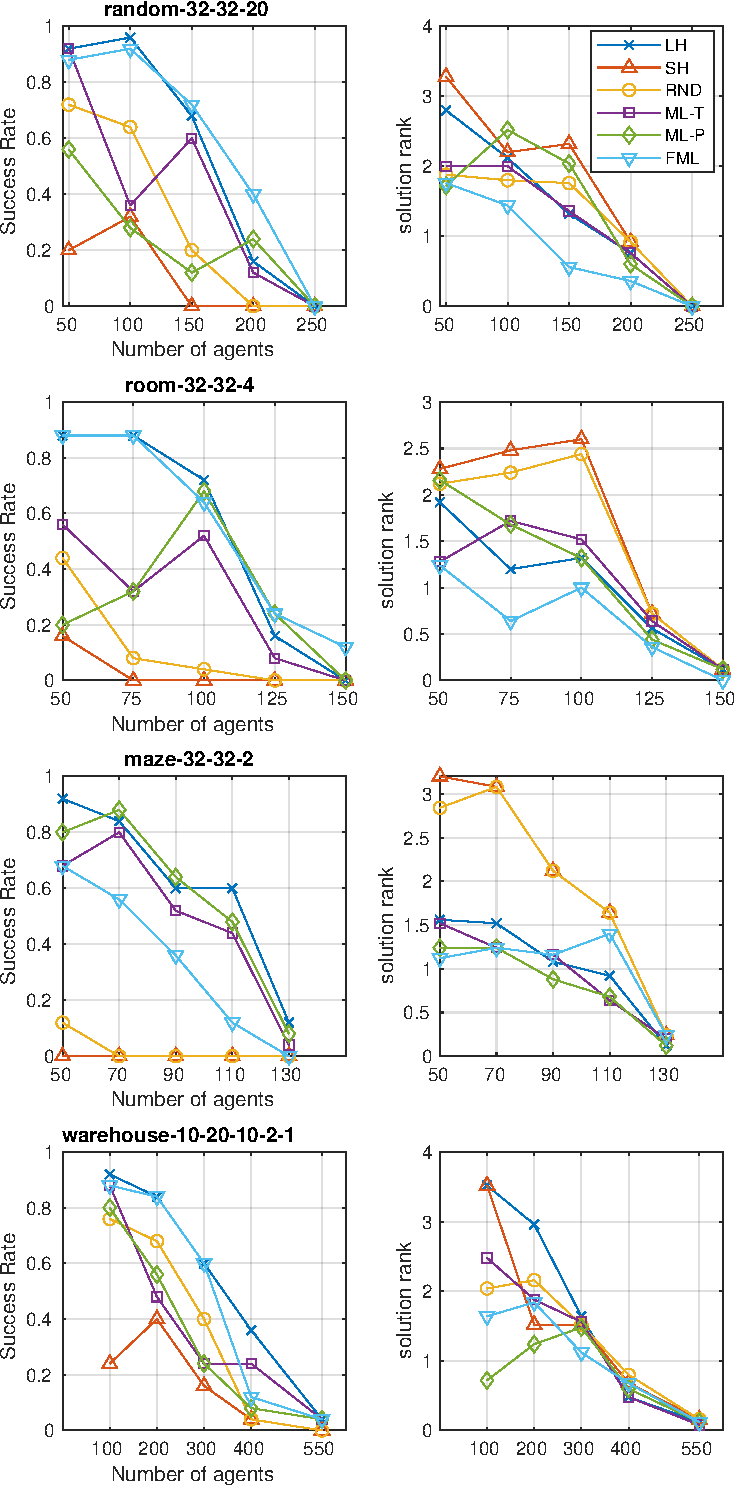
\includegraphics[width=1.0\columnwidth]{figs/succRankPortability.pdf}
\caption{Success rate and average solution rank of $ f_{} $  }
\label{fig:portability}
\end{figure}

We will now evaluate performance of $ f_{} $ on the three small maps and the one medium sized map with deterministic ranking to demonstrate an example of the formula's portability. Instead of computing the agents' priority scores using the formulae synthesized specifically for that number of agents and that map, we use $ f_ $ on all the maps and with all numbers of agents. As per Figure~\ref{fig:portability} the formula $ f_ $ has the highest success rate and the best average solution rank for most numbers of agents on {\tt random-32-32-20} and {\tt room-32-32-4}. It performs worse on {\tt maze-32-32-2} and {\tt warehouse-10-20-10-2-1}. This shows that the synthesized formulae can  

%%%%%%%%%%%%%%%%%%%%%%%%%%%%%%%%%%%%%%%%%%%%%%%%%%%
\section{Future Work}

     ously synthesized formulae~\cite{bulitko2022portability}, leading   training sets by using other synthesis methods~\citep{shah2022near,mapElites,Gallotta_2022,FI2Pop}.

%%%%%%%%%%%%%%%%%%%%%%%%%%%%%%%%%%%%%%%%%%%%%%%%%%%
\section{Conclusions}
\label{sec:conclusions}

We adopted the approach by~\citet{bulitko2022portability} to learn priority to solve multi-agent pathfinding problems   search. They are short and human-readable and  ap 

We also showed that our synthesized formula can outperform existing PP algorithms in both success rate and   

\section*{}



\clearpage
\bibliography{aiide2023}

\end{document}
